%%
% This is an Overleaf template for presentations
% using the TUM Corporate Desing https://www.tum.de/cd
%
% For further details on how to use the template, take a look at our
% GitLab repository and browse through our test documents
% https://gitlab.lrz.de/latex4ei/tum-templates.
%
% The tumbeamer class is based on the beamer class.
% If you need further customization please consult the beamer class guide
% https://ctan.org/pkg/beamer.
% Additional class options are passed down to the base class.
%
% If you encounter any bugs or undesired behaviour, please raise an issue
% in our GitLab repository
% https://gitlab.lrz.de/latex4ei/tum-templates/issues
% and provide a description and minimal working example of your problem.
%%

\PassOptionsToClass{onlytextwidth}{beamer}

\documentclass[
  german,            % define the document language (english, german)
  aspectratio=169,    % define the aspect ratio (169, 43)
  % handout=2on1,       % create handout with multiple slides (2on1, 4on1)
  % partpage=false,     % insert page at beginning of parts (true, false)
  % sectionpage=true,   % insert page at beginning of sections (true, false)
]{tumbeamer}


% load additional packages
\usepackage{booktabs}
\usepackage{graphicx}
\usepackage{tikz}
\usepackage{url}
\usepackage{pgfplots}
\usepackage{hyperref}
\usepackage{pmboxdraw}
\usepackage{float}
\usepackage{babel}[ngerman]
\usepackage{csquotes}[autostyle]
\usepackage[useregional]{datetime2}
\usepackage[cache=true]{minted}

% tikz
\usetikzlibrary{arrows,arrows.meta,backgrounds,positioning,shapes,patterns,patterns.meta,matrix,arrows.meta,shapes.geometric,decorations.pathmorphing, matrix, fit, calc, overlay-beamer-styles}

% minted
\setminted{
	fontsize=\small, 
	frame=single,
	breaklines=true,
	style=vs,
	tabsize=4, 
	autogobble,
}

% image path
\graphicspath{ {./resources/} }

% beamer
\setbeamercolor{footnote}{fg=black}
\setbeamercolor{footnote mark}{fg=black}
\renewcommand{\thempfootnote}{\arabic{mpfootnote}}

% presentation metadata
\title{Übung 03: Sprünge und Pointer}
\subtitle{Einführung in die Rechnerarchitektur}
\author{Niklas Ladurner}

\institute{\theChairName\\\theDepartmentName\\\theUniversityName}
\date{\DTMdisplaydate{2025}{10}{31}{-1}}

\footline{\insertauthor~|~\insertshorttitle~|~\insertshortdate}


% macro to configure the style of the presentation
\TUMbeamersetup{
  title page = TUM tower,         % style of the title page
  part page = TUM toc,            % style of part pages
  section page = TUM toc,         % style of section pages
  content page = TUM more space,  % style of normal content pages
  tower scale = 1.0,              % scaling factor of TUM tower (if used)
  headline = TUM threeliner,      % which variation of headline to use
  footline = TUM default,         % which variation of footline to use
  % configure on which pages headlines and footlines should be printed
  headline on = {title page},
  footline on = {every page, title page=false},
}

% available frame styles for title page, part page, and section page:
% TUM default, TUM tower, TUM centered,
% TUM blue default, TUM blue tower, TUM blue centered,
% TUM shaded default, TUM shaded tower, TUM shaded centered,
% TUM flags
%
% additional frame styles for part page and section page:
% TUM toc
%
% available frame styles for content pages:
% TUM default, TUM more space
%
% available headline options:
% TUM empty, TUM oneliner, TUM twoliner, TUM threeliner, TUM logothreeliner
%
% available footline options:
% TUM empty, TUM default, TUM infoline


\begin{document}

\maketitle

\begin{frame}[c]{}{}
	\begin{center}
		\LARGE  Keine Garantie für die Richtigkeit der Tutorfolien.

		\Large Bei Unklarheiten/Unstimmigkeiten haben VL/ZÜ-Folien recht!
	\end{center}
\end{frame}

\begin{frame}[c, fragile]{Sprungbefehle}{}
	\vspace{-0.5cm}
	\begin{columns}
		\begin{column}{0.5\textwidth}
			\begin{center}\textbf{Branch-Befehle}\end{center}
			Rücksprungadresse wird nicht gesichert, \textbf{Sprungbedingung}
			muss erfüllt sein
			\vspace{0.5\baselineskip}
			\begin{itemize}
				\item \verb|beq|: $rs1 = rs2$
				\item \verb|bne|: $rs1 \ne rs2$
				\item \verb|blt(u)|: $rs1 < rs2$
				\item \verb|bgt(u)|: $rs1 > rs2$
			\end{itemize}
			\begin{center}
				\underline{für Schleifen und Bedingungen (if's)}
			\end{center}
		\end{column}
		\begin{column}{0.5\textwidth}
			\begin{center}\textbf{Jump-Befehle}\end{center}
			Schreiben Rücksprungadresse in \texttt{ra} oder angegebenes Register,
			springen immer
			\vspace{0.5\baselineskip}
			\begin{itemize}
				\item \verb|jal label|
				\item \verb|jalr rd, offset(rs)|
				\item \verb|call label| \footnote[frame]{Pseudobefehl für \texttt{jalr} mit 32-Bit Offset}
				\item \verb|j label| (Überschreibt \texttt{ra} nicht)
			\end{itemize}
			\begin{center}
				\underline{für Rekursion und Unterprogramme\footnote[frame]{außer \texttt{j label}, Pseudobefehl für \texttt{jal zero, label}}}
			\end{center}
		\end{column}
	\end{columns}
\end{frame}

\begin{frame}[c, fragile]{Speichermodell}{}
	\begin{columns}
		\begin{column}{0.65\textwidth}
			\begin{itemize}
				\item 32-Bit-Architektur, d.h. Wortbreite von 4 Byte
				\item Adressen folglich auch 32 Bit
				\item Speicher ist Byte-addressierbar
				\item Daten liegen nacheinander im Speicher
				\item Adresse eines Symbols kann mittels \texttt{la rd, sym} geladen werden
			\end{itemize}
		\end{column}
		\begin{column}{0.35\textwidth}
			\begin{center}
				\begin{minted}{c}
					struct myStruct{
						int x;
						char y;
						char z;
					};
				\end{minted}
			\end{center}
		\end{column}
	\end{columns}
	\begin{figure}
		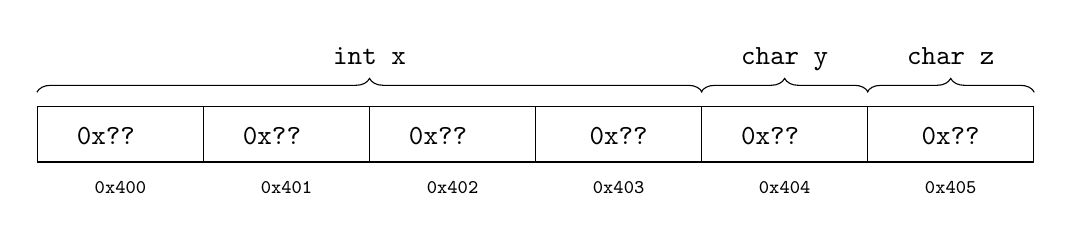
\begin{tikzpicture}
			\tikzset{
				label/.style = {font={\ttfamily}},
				arrow/.style={->, thick},
				matstyle/.style={ matrix of nodes, ampersand replacement=\&, nodes={draw, minimum width=6em, minimum height=2em, text height=1em, text depth=0.25em, align=center, anchor=south}, column sep=-\pgflinewidth, font={\ttfamily}},
			}


			\matrix[matstyle] (mat) {
				0x?? \& 0x?? \& 0x?? \& 0x??\& 0x?? \& 0x??%
				\\
			};

			\draw [decorate,decoration={brace,amplitude=5pt,raise=0.5em}]
			(mat-1-1.north west) -- (mat-1-4.north east) node[midway,yshift=2em, text height=1em, text depth=0em]{\texttt{int x}};

			\draw [decorate,decoration={brace,amplitude=5pt,raise=0.5em}]
			(mat-1-5.north west) -- (mat-1-5.north east) node[midway,yshift=2em, text height=1em, text depth=0em]{\texttt{char y}};

			\draw [decorate,decoration={brace,amplitude=5pt,raise=0.5em}]
			(mat-1-6.north west) -- (mat-1-6.north east) node[midway,yshift=2em, text height=1em, text depth=0em]{\texttt{char z}};

			\foreach \x in {1, 2, 3, 4, 5, 6}
				{
					\node[label, font=\ttfamily\scriptsize, below=0.125cm of mat-1-\x.south, anchor=north] (addr) {0x\fpeval{400+\x-1}};
				}

		\end{tikzpicture}
	\end{figure}
\end{frame}

\begin{frame}[c, fragile]{Sections und Direktiven}
	\begin{columns}[c]
		\begin{column}{0.49\textwidth}
			\begin{minted}{gas}
				# compile-time Konstante
				.equ NUM, 2748 
				
				# ro + init. Daten
				.rodata
				f: .word 2
				
				# rw + init. Daten
				.org 0x400
				.data
				arr: .byte 4, 3, 2, 1
				string1: .ascii "asdf"
				string2: .asciz "asdf"
			\end{minted}
		\end{column}
		\begin{column}{0.49\textwidth}
			\begin{minted}{gas}
				# rw + uninit. Daten
				.bss
				a: .space 16
				
				# globales Einstiegslabel
				.globl _start
				
				.org 0x200 # section beginnt an Adresse 0x200
				.text
				_start:
				la a0, arr
				lbu a1, 0(a0)
			\end{minted}
		\end{column}
	\end{columns}
	\begin{center}
		\small{\textbf{ro}: read-only, \textbf{rw}: les- und schreibbar}
	\end{center}
\end{frame}

\begin{frame}[c]{Byte-Reihenfolge (Endianness)}{}
	\begin{center}
		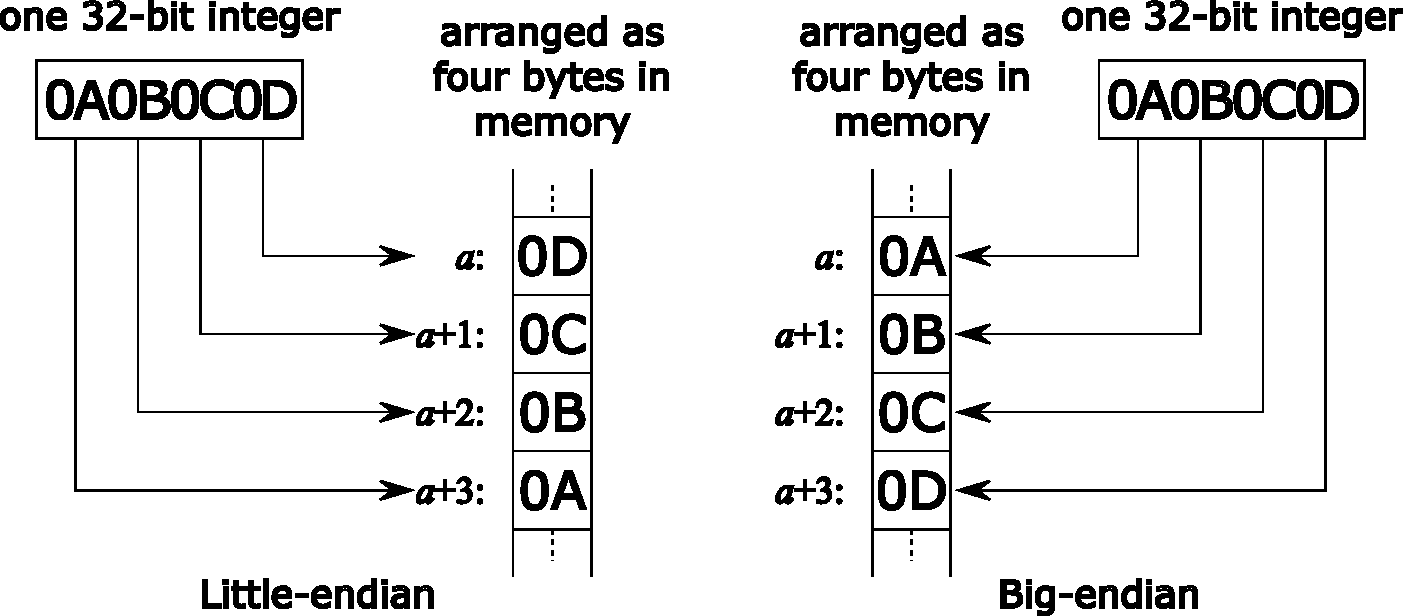
\includegraphics[width=0.8\textwidth]{w03_endianess.pdf}
	\end{center}
\end{frame}

\begin{frame}[c, fragile]{Byte-Reihenfolge (Endianness)}{}
	\vspace{-0.5cm}
	\begin{columns}[c]
		\begin{column}{0.45\textwidth}
			\vspace{1.5cm}
			\begin{minted}[escapeinside=||, beameroverlays=true,]{gas}
				.org 0x400
				.data
				
				|\only<1>{a: .byte \textcolor{red}{0x01}, \textcolor{orange}{0x02}, \textcolor{green}{0x03}, \textcolor{blue}{0x04}}\only<2->{a: .byte 0x01, 0x02, 0x03, 0x04}|
				|\only<2>{b: .half 0x\textcolor{red}{ab}\textcolor{orange}{cd}, 0x\textcolor{green}{00}\textcolor{blue}{ef}}\only<3->{b: .half 0xabcd, 0x00ef}|
				|\only<3>{c: .word 0x\textcolor{red}{aa}\textcolor{orange}{bb}\textcolor{green}{cc}\textcolor{blue}{dd}}\only<4->{c: .word 0xaabbccdd}|
			\end{minted}
			\vspace{0.5\baselineskip}
			\textbf{Wichtig}: Innerhalb der einzelnen Bytes bleibt die Bitreihenfolge gleich!
		\end{column}
		\begin{column}{0.55\textwidth}
			\centering
			\begin{figure}
				\resizebox{\textwidth}{!}{
					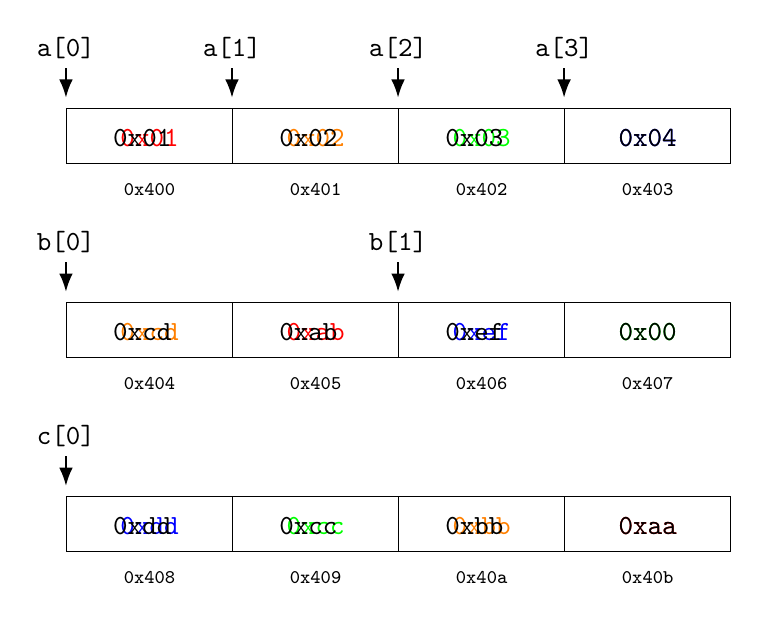
\begin{tikzpicture}
						\tikzset{
							label/.style = {font={\ttfamily}},
							arrow/.style={-Latex, thick},
							matstyle/.style={ matrix of nodes, ampersand replacement=\&, nodes={draw, minimum width=6em, minimum height=2em, text height=1em, text depth=0.25em, align=center, anchor=south}, column sep=-\pgflinewidth, font={\ttfamily}},
						}

						\def\lblspc{0.5cm}
						\def\matspc{1.5cm}


						\uncover<1->{
							\matrix[matstyle, visible on=<1>] (mat1) {
								\textcolor{red}{0x01}\&\textcolor{orange}{0x02}\&\textcolor{green}{0x03}\&\textcolor{blue}{0x04}%
								\\
							};
							\matrix[matstyle, visible on=<2->] (mat1) {
								0x01 \& 0x02 \& 0x03 \& 0x04%
								\\
							};
							\foreach \x in {1, 2, 3, 4}
								{
									\node[label, above=\lblspc of mat1-1-\x.north west] (ptr) {a[\fpeval{\x-1}]};
									\node[label, font=\ttfamily\scriptsize, below=0.125cm of mat1-1-\x.south, anchor=north] (addr) {0x\fpeval{400+\x-1}};
									\draw[arrow] (ptr) -- ($(mat1-1-\x.north west) + (0, 0.125)$);
								}
						}

						\uncover<2->{
							\matrix[matstyle, below=\matspc of mat1, visible on=<2>] (mat2) {
								\textcolor{orange}{0xcd}\&\textcolor{red}{0xab}\&\textcolor{blue}{0xef}\&\textcolor{green}{0x00}%
								\\
							};
							\matrix[matstyle, below=\matspc of mat1, visible on=<3->] (mat2) {
								0xcd \& 0xab \& 0xef \& 0x00%
								\\
							};
							\foreach \x in {1,3}
								{
									\node[label, above=\lblspc of mat2-1-\x.north west] (ptr) {b[\fpeval{(\x-1)/2}]};
									\draw[arrow] (ptr) -- ($(mat2-1-\x.north west) + (0, 0.125)$);
								}

							\foreach \x in {1,2,3,4}{
									\node[label, font=\ttfamily\scriptsize, below=0.125cm of mat2-1-\x.south, anchor=north] (addr) {0x\fpeval{404+\x-1}};}
						}

						\uncover<3->{
							\matrix[matstyle, below=\matspc of mat2, visible on=<3>] (mat3) {
								\textcolor{blue}{0xdd}\&\textcolor{green}{0xcc}\&\textcolor{orange}{0xbb}\&\textcolor{red}{0xaa}%
								\\
							};

							\matrix[matstyle, below=\matspc of mat2, visible on=<4->] (mat3) {
								0xdd \& 0xcc \& 0xbb \& 0xaa%
								\\
							};

							\node[label, above=\lblspc of mat3-1-1.north west] (ptr) {c[0]};
							\draw[arrow] (ptr) -- ($(mat3-1-1.north west) + (0, 0.125)$);

							\foreach \x/\v in {1/8,2/9,3/a,4/b}{
									\node[label, font=\ttfamily\scriptsize, below=0.125cm of mat3-1-\x.south, anchor=north] (addr) {0x40\v};}
						}
					\end{tikzpicture}
				}
			\end{figure}
		\end{column}
	\end{columns}
\end{frame}

\begin{frame}[c, fragile]{Speicherzugriffe\footnote{\textbf{b}yte: 1 Byte, \textbf{h}alf-word: 2 Byte, \textbf{w}ord: 4 Byte}}{}
	\begin{columns}[c]
		\begin{column}{0.5\textwidth}
			\begin{center}
				\only<1-3>{
					{\Large\ttfamily lw t0, 0(a0)}

					\vspace{\baselineskip}
					lade 4 Byte an der Adresse \texttt{a0} + 0 Bytes Offset in das Register \texttt{t0}
				}

				\only<4-6>{
					{\Large\ttfamily lb t1, -4(a2)}

					\vspace{\baselineskip}
					lade 1 Byte (sign-extended) an der Adresse \texttt{a2} - 4 Bytes Offset in das Register \texttt{t1}
				}

				\only<7-9>{
					{\Large\ttfamily sh t3, 2(t4)}

					\vspace{\baselineskip}
					speichere die unteren 2 Byte von \texttt{t3} an der Adresse \texttt{t4} + 2 Bytes Offset
				}
			\end{center}
		\end{column}
		\begin{column}{0.5\textwidth}
			\begin{center}
				\begin{figure}
					\begin{tikzpicture}
						\tikzset{
							label/.style = {font={\ttfamily\scriptsize}},
							biglabel/.style = {font={\ttfamily\normalsize}},
							arrow/.style={Latex-, thick},
							matstyle/.style={ matrix of nodes, ampersand replacement=\&, nodes={draw, minimum width=6em, minimum height=2em, text height=1em, text depth=0.25em, align=center, anchor=south}, row sep=-\pgflinewidth, font={\ttfamily}},
							bbox/.style={fill=TUMBlue, draw=TUMBlue, semitransparent, rounded corners, thick, inner sep=-2pt},
							bbrace/.style={decorate,decoration={brace,amplitude=5pt,raise=0.5em}, rotate=90, thick},
						}

						\only<1-8>{
							\matrix[matstyle] (mat) {
								0x01%
								\\0x02%
								\\0x03%
								\\0x04%
								\\0x05%
								\\0x06%
								\\
							};
						}

						\only<9>{
							\matrix[matstyle] (mat) {
								0x01%
								\\0x02%
								\\0x03%
								\\0x04%
								\\0xdd%
								\\0xcc%
								\\
							};
						}

						\foreach \x in {1, 2, 3, 4, 5, 6}
							{
								\node[label, left=0.125cm of mat-\x-1.north west, anchor=east] (addr) {0x\fpeval{400+\x-1}};
							}

						\only<1-3>{
							\node[biglabel, below=0.5cm of mat] {a0 = 0x00000401};
							\draw[arrow, visible on=<1>] (mat-2-1.north east) -- ++(0.5cm, 0);
							\pause

							\draw [bbrace] (mat-2-1.north east) -- (mat-5-1.south east) node[midway,xshift=2em,biglabel]{lw};
							\pause

							\node[bbox, fit=(mat-2-1.north west) (mat-5-1.south east)] {};
							\node[biglabel, below=1cm of mat] {t0 = 0x05040302};
						}

						\only<4-6>{
							\node[biglabel, below=0.5cm of mat] {a2 = 0x00000404};
							\draw[arrow, visible on=<4>] (mat-5-1.north east) -- ++(0.5cm, 0);
							\pause\pause\pause

							\draw[arrow, blue, visible on=<4>] (mat-1-1.north east) -| node[biglabel, pos=0.75, right] {\texttt{-4}} ($(mat-5-1.north east) +(0.5cm, 0)$);

							\pause

							\draw[bbrace] (mat-1-1.north east) -- (mat-1-1.south east) node[midway,xshift=2em,biglabel]{lb};
							\pause

							\node[bbox, fit=(mat-1-1.north west) (mat-1-1.south east)] {};
							\node[biglabel, below=1cm of mat] {t1 = 0x00000001};
						}

						\only<7-9>{
							\node[biglabel, below=0.5cm of mat] {t4 = 0x00000402};
							\node[biglabel, below=1cm of mat] {t3 = 0xaabbccdd};
							\draw[arrow, visible on=<7>] (mat-3-1.north east) -- ++(0.5cm, 0);
							\draw[arrow, blue, visible on=<7>] (mat-5-1.north east) -| node[biglabel, pos=0.75, right] {+2}  ($(mat-3-1.north east)+(0.5cm, 0)$);
							\pause\pause\pause\pause\pause\pause\pause

							\draw [bbrace] (mat-5-1.north east) -- (mat-6-1.south east) node[midway,xshift=2em,biglabel]{sh};
							\pause

							\node[bbox, fit=(mat-5-1.north west) (mat-6-1.south east)] {};
						}
					\end{tikzpicture}
				\end{figure}
			\end{center}
		\end{column}
	\end{columns}
\end{frame}

\begin{frame}[c]{}{}
	\begin{center}
		\LARGE Fragen?
	\end{center}
\end{frame}


\begin{frame}[c, fragile]{Links}{}
	\begin{itemize}
		\item Zulip: \href{https://zulip.in.tum.de/#narrow/channel/3255-ERA-Tutorium-.E2.80.93-Mi-1600-3}{\enquote{ERA Tutorium -- Mi-1600-3}}
		      bzw. \href{https://zulip.in.tum.de/#narrow/channel/3264-ERA-Tutorium-.E2.80.93-Fr-1500-1}{\enquote{ERA Tutorium -- Fr-1500-1}}
		\item \href{https://www.moodle.tum.de/course/view.php?id=111440}{ERA-Moodle-Kurs}
		\item \href{https://artemis.in.tum.de/courses/516}{ERA-Artemis-Kurs}
		\item \href{https://msyksphinz-self.github.io/riscv-isadoc/html/index.html}{Übersicht an RISC-V-Instruktionen}
		\item \href{https://ftp.gnu.org/old-gnu/Manuals/gas/html_chapter/as_7.html}{GNU as directives}
	\end{itemize}
\end{frame}

\maketitle

\end{document}
